\documentclass{report}
% Comment the following line to NOT allow the usage of umlauts
\usepackage[utf8]{inputenc}
\usepackage[left=3cm,right=3cm,top=3.5cm,bottom=3.5cm]{geometry}
\usepackage[francais]{babel}
\usepackage{listings}
\usepackage{xcolor}
\usepackage{textcomp}
\pagestyle{plain}
\definecolor{listinggray}{gray}{0.9}
\definecolor{lbcolor}{rgb}{0.9,0.9,0.9}
\definecolor{darkWhite}{rgb}{0.94,0.94,0.94}
\lstset{
aboveskip=3mm,
belowskip=3mm,
backgroundcolor=\color{darkWhite},
basicstyle=\footnotesize,
breakatwhitespace=false,
breaklines=true,
captionpos=b,
commentstyle=\color{red},
deletekeywords={...},
escapeinside={\%*}{*)},
extendedchars=true,
framexleftmargin=16pt,
framextopmargin=3pt,
framexbottommargin=6pt,
frame=tb,
keepspaces=true,
keywordstyle=\color{blue},
language=C,
literate=
{²}{{\textsuperscript{2}}}1
{⁴}{{\textsuperscript{4}}}1
{⁶}{{\textsuperscript{6}}}1
{⁸}{{\textsuperscript{8}}}1
{€}{{\euro{}}}1
{é}{{\'e}}1
{è}{{\`{e}}}1
{ê}{{\^{e}}}1
{ë}{{\¨{e}}}1
{É}{{\'{E}}}1
{Ê}{{\^{E}}}1
{û}{{\^{u}}}1
{ù}{{\`{u}}}1
{â}{{\^{a}}}1
{à}{{\`{a}}}1
{á}{{\'{a}}}1
{ã}{{\~{a}}}1
{Á}{{\'{A}}}1
{Â}{{\^{A}}}1
{Ã}{{\~{A}}}1
{ç}{{\c{c}}}1
{Ç}{{\c{C}}}1
{õ}{{\~{o}}}1
{ó}{{\'{o}}}1
{ô}{{\^{o}}}1
{Õ}{{\~{O}}}1
{Ó}{{\'{O}}}1
{Ô}{{\^{O}}}1
{î}{{\^{i}}}1
{Î}{{\^{I}}}1
{í}{{\'{i}}}1
{Í}{{\~{Í}}}1,
morekeywords={*,...},
numbers=left,
numbersep=10pt,
numberstyle=\tiny\color{black},
rulecolor=\color{black},
showspaces=false,
showstringspaces=false,
showtabs=false,
stepnumber=1,
stringstyle=\color{gray},
tabsize=4,
title=\lstname,
}

\title{Rapport de TER}
% Start the document
\begin{document}
\maketitle
\newpage
\tableofcontents
\newpage
% Create a new 1st level heading

\part{Présentation du projet}
\chapter{Introduction}
\section{But du projet}
\paragraph{}
L'objectif de ce projet est la réalisation d'un jeu basé sur un modèle multi-agent. L'idée générale du projet est dans la continuité de celui de l'année dernière et sur le même thème. L'outil utilisé est Unity 3D, un moteur de jeu employé dans un grand nombre de réalisations de hautes qualités. Notre projet est opérationnel sur Windows et pourrait être porté sur Mac ou encore Android.
Ce projet consiste de réaliser un jeu que l'on peut qualifier de programmeur et de permettre, notamment, à de jeunes personnes de se familiariser avec le monde de la programmation. L'utilisateur pourra donc créer un comportement pour des robots appelés "unité" afin de remplir des objectifs du jeu.
\paragraph{}
Metabot est un projet modeste réalisé à partir du logiciel Unity 3D par un groupe d'étudiants débutants dans l'utilisation de cet outil. Malgré le peu d'expérience dans la création pure de ce genre d'applications, le projet actuel est le fruit d'un travail important et d'une implication entière de toute l'équipe.
Il a donc pour unique prétention de communiquer notre amour du jeu vidéo et de la programmation.

\section{Cahier des charges}

Notre but était de modifier le programme existant afin qu'il devienne plus générique. C'est à dire qu'il ne se limite plus au simple jeu Warbot mais qu'il permette l'implémentation de différents jeux orientées agents facilement. 
Pour cela il fallait donc généraliser la gestion des différentes unités et de leur comportement (action/perception/statistique). De plus, l'ajout d'actions et de moyens de perceptions doit se faire de façon intuitive de même pour les différentes exigences de jeu (règles/conditions de victoire). 

\section{Notion d'agent}

\subsection{Système multi-agents}

\subsection{Representation dans notre projet}

\newpage

\chapter{WarBot: Le mode par défaut}
\section{Principe}
Dans WarBot, deux à quatre équipes se battent sur un terrain pour les ressources afin de survivre et d'éliminer les autres équipes et d’être la dernière ne vie. Des ressources apparaissent sur la carte et peuvent être converties en unités ou en soin.

\newpage
\part{Réalisation du projet}
\newpage

%%%
% PARTIE MOTEUR
%%%
\chapter{Partie "Moteur"}

\section{État de l'art de l'ancien projet.} Mehdi

\section{Refonte du noyau.}
\paragraph{}L'ancien projet est une adaptation du jeu Warbot crée en java en utilisant la librairie MadKit, permettant la conception et la simulation de système multi-agents. En utilisant comme base ce projet, et en utilisant la hiérarchie de classe proposé dans le code java dans un moteur de jeu relativement bien assisté comme Unity, de nombreux problèmes de conceptions peuvent apparaître.
\paragraph{}Unity, pour rappel, est un moteur de jeu développé par Unity Technologies. Ce logiciel à la particularité d'etre "orienter assets". Les scripts associé à chaque objet (appellée GameObject) dérive de la classe "MonoBehaviour", ce qui permet d'avoir accées à un ensemble de méthodes et d'attribut nécessaire à la création de comportement et d'interaction.
\paragraph{} Dans cette section, nous allons développer les problèmes que nous avons rencontrer dans la réalisation d'un moteur de jeu générique sur la base de l'ancien projet et de l'explication de la nécessiter de recréer un moteur à partir de zéro.
\paragraph{} Nous avons donc remarqué des problèmes du faite de ce choix de conception. Tout abords les scripts en eux-même ne sont pas adaptés au développement d'un programme sur Unity et surtout ne sont pas générique.  En effet, les unités sont codés en dur dans le code, ne permettant pas l'ajout de nouvelles unités de façon simple. Ainsi pour rajouter de nouvelles unités, il faut créer de nouvelles classes correspondant a de nouvelles unités. Cette hiérarchie des classes est un parti-pris que l'équpe de l'année passée à choisi en se basant sur le code java de WarBot. Cependant, la problématique de notre sujet de TER ne nous permet pas d'avoir ce genre de conception dans l'idée de rendre l'ajout des unités plus simple. Ainsi, il fallait reprendre la conception des unités et voir les composants que l'on peut garder de façon unique et modulable pour toute les unités.
%% DEBUT CODE %%
\begin{lstlisting}[language={[Sharp]C}, caption= Code du script AttackController.cs de l'ancien projet]
using System.Collections;
using System.Collections.Generic;
using UnityEngine;
using System;
using WarBotEngine.Projectiles;
using System.Security.Cryptography;

namespace WarBotEngine.WarBots {

    public class AttackController : MonoBehaviour {
[...]
        public bool Reloaded()
        {
            return (this.reloading + this.reload_time < Time.time);
        }

        public bool Shoot()
        {
            if (!this.Reloaded())
                return false;
            this.Fire();
            return true;
        }
[...]
        public void Fire() {
            SoundManager.Actual.PlayFire(this.gameObject);
            Instantiate(this.projectile , this.warprojectile_emitter.transform.position , this.warprojectile_emitter.transform.rotation , this.transform);
            Instantiate(this.muzzle_flash , this.warprojectile_emitter.transform.position , this.warprojectile_emitter.transform.rotation , this.transform);
            this.reloading = Time.time;
        }
    }
}
\end{lstlisting}

\paragraph{} La gestion des actions et des perceptions aussi est problématique. Le code de ces actions sont codés en dur dans des scripts correspondant a des unités d'un certain type, empêchant alors de rendre générique le fait de rajouter des actions sans devoir modifier tout les codes nécessitant le nom des actions tel que l’interpréteur. Le code ci-dessous montre le script "AttackController.cs" de l'ancien projet. Dans ce code, l'actions Shoot depend des fonction Reloaded et Fire. Reloaded peut être considérer comme une perception. Le fait que les actions et les perceptions ne sont pas clairement définie entant que tels posent des problèmes de compréhension du code et de faite le rajout de façon simple une nouvelle action et une nouvelle perception. De plus, cela pose le problème de la gestion des actions et des perceptions de l’interpréteur, car pour chaque action créer dans le script, il faut indiquer à l'interpreteur quelle fonction permet d'activer l'action du comportement en cours. 
\paragraph{}Ainsi dans le code du listing \ref{lst:unitScript}, on peut voir que pour activer la fonction Shoot() du script AttackController, il faut créer une fonction du même nom, puis renseigner toutes les unités qui peuvent effectuer l'action. Le problème est qu'il faut, pour chaque action, créer une fonction dans le fichier Unit.cs, et ainsi le fichier Unit.cs est surchargé, atteignant les 2000 lignes de codes !

\begin{lstlisting}[language={[Sharp]C},label={lst:unitScript}, caption=  Extrait du code du script Unit.cs]
using ...;
namespace WarBotEngine.Editeur
{
   [...]
	public class Unit
    {
        /// <summary>
        /// The unit shoot a projectile if is reloading
        /// </summary>
        /// <returns>Return true if action success and false otherwise</returns>
        [PrimitiveType(PRIMITVE_TYPE.ACTION)]
        [UnitAllowed(WarBots.BotType.WarHeavy)]
        [UnitAllowed(WarBots.BotType.WarTurret)]
        [PrimitiveDescription("Fait tirer l'unité (termine l'action si réussi)")]
        public bool Shoot()
        {
            return this.agent.GetComponent<WarBots.AttackController>().Shoot();
        }
   }
}

\end{lstlisting}
\paragraph{} La suite de l'examen du code de l'ancien projet et avec l'accord de notre encadrant en exposant les problèmes qu'engendre la reprise de l'ancien moteur, nous avons décider de recréer un nouveau moteur de jeu pour repartir sur des bases plus générique.


\section{Réalisation}


\subsection{Retour aux bases.} Mehdi
\subsection{Intégration dans le projet.}
\subsubsection{La phase d'intégration.} Maxime
\subsubsection{Problèmes liés à l'intégration.} Maxime
\subsubsection{Résolution des problèmes.} Maxime



\subsection{Améliorations des fonctionnalités.}
\subsubsection{Optimisation du temps de chargement}
\paragraph{} L'un des gros problèmes que l'on a rencontré est le fait que le temps de chargement lors d'une partie était beaucoup trop élevé et cela nuisait au bon déroulement de la partie, atteignant parfois deux minutes de temps de chargement lorsque l'on voulait générer 200 unités. Pour ce la nous avons étudier plusieurs pistes pour résoudre ce problème
\subparagraph{La gestion des actions des unités.}La premier piste de recherche que l'on a étudié est d'essayer d'optimiser la gestion des actions des unités. Lorsque l'on a conçu les unités, elle faisaient leurs actions dans une fonction utilisé par Unity "Update" qui est appelé à chaque calcul d'image. Ainsi pour chaque unités présente sur la scène, Unity calcule l'action que l'unité doit faire. Cependant, certaine action nécessite plus de temps en fonction de sa complexité, ce qui pouvait engendré que des unités avaient des tours de retard par rapport à d'autres unités. \newline
Pour palier à ce problème, nous avons donc délégué à un script  "TurnManagerScript.cs" (Listing \ref{lst:turnManagerScript}) la gestion des unités.\newline
 \begin{lstlisting}[language={[Sharp]C},label={lst:turnManagerScript}, caption= Code du script TurnManagerScript.cs]
using System.Collections;
using System.Collections.Generic;
using UnityEngine;

public class TurnManagerScript : MonoBehaviour
{
    public float _timeTick;
    public float _ticksPerSeconds;
    
    // Update is called once per frame
	void FixedUpdate ()
    {
        _timeTick += 0.02F * Time.timeScale;
        _ticksPerSeconds = (1.0f / 0.02F) * Time.timeScale;
        if (_timeTick >= 0.04f) // Est-ce que 0.4 secondes ce sont écoulées ?
        {
            _timeTick -= 0.04f;

            foreach (GameObject unit in GameObject.FindGameObjectsWithTag("Unit"))
            {
                if (unit.GetComponent<Brain>()) // Comporte un "Brain"
                {
                    unit.GetComponent<Brain>().UnitTurn(); // Fait l'action de l'unité
                }
            }
        }
	}
}
\end{lstlisting}
Ce script permet donc de controler que chaque unité ne commence pas un nouveau tour si d'autre unité n'ont pas fini ou fait le leur.
Cependant, cette optimisation n'a pas permis de réduire le temps de chargement d'une partie, restant toujours à prés de deux minutes pour la génération de 200 unités.

\subparagraph{\textit{ObjectPool}, les "bassins" d'objets.}Pour essayer de mieux localiser le problème, nous avons effectuer des tests sur le temps de chargement en fonction du nombre d'unités. Les résultats sont consignés dans le tableau ci-dessous. On peut donc voir que le nombre d'unité à générer influe directement le temps de chargement.\newline
\begin{center}
\begin{tabular}{c|c}
  \hline
  Nombre d'unités à générer & Temps de chargements (moyenne de 3 tests) \\
  \hline
  0 unités & 0.49 secondes \\
  1 unités & 0.70 secondes \\
  5 unités & 3.13 secondes \\
  20 unités & 11.50 secondes \\
  50 unités & 27.84 secondes \\
  100 unités & 50.23 secondes \\
  200 unités & 162.20 secondes \\
  500 unités & 276.71 secondes \\
  \hline
\end{tabular}
\end{center}
Pour empêcher la génération des unités pendant lors du chargement, nous décidons d'utiliser une méthode dite "du bassins d'objets" (ou \textit{ObjectPooling}). Cette méthode consiste à créer un ensemble d'objet dans un objet appelé \textit{Pool}, puis de les rendre inactifs pour que les scripts contenu dans ces objets ne soient pas exécutés.

%% CODE %%
 \begin{lstlisting}[language={[Sharp]C},label={lst:structPoolScript}, caption= Code de la structure \textit{Pool} de ObjectPool.cs]
public struct Pool
{
    public string tag; // Label du Pool
    public int number; // Nombre d'objets
    public GameObject prefab; //Objet de référence
}
\end{lstlisting}

Cette méthode permet de ne pas créer une unité directement, mais de juste prendre un objet Unit dans le bassin correspondant. Les bassins sont représentes par une structure définit au listing \ref{lst:structPoolScript}. elle comporte un \textit{tag} représentant le nom du bassin, un  \textit{number} correspondant au nombre d'unités à créer dans ce bassin, et enfin un \textit{prefab} qui est l'objet qui servira de référence pour la copie des objets. Le script gérant le script (Listing  \ref{lst:ObjectPoolScript}) permet la gestion de plusieurs \textit{Pools}, et dans notre cas, nous utilisons 3 \textit{Pools}:  \textit{Light},  \textit{Heavy} et  \textit{Explorer}


\subsection{Fonctionalités finales.}
Mehdi
\section{Amélioration possible}
Mehdi et Maxime
\subsection{Gestion des unités.}

La gestion des unités de manière générique nous a poussé à réfléchir aux éléments minimum définissant celle-ci.
Elles nécessitent donc 6 scripts de base : 
\begin{itemize}
\item Brain
\item Stats
\item Percept
\item Actions
\item ActionNonTerminales
\item Messages
\end{itemize}

\subsubsection{Le corps}

Le corps de l'unité correspond à son modèle 3D, et son GameObejct Collider associé.

Pour le jeu warbot nous avons réaliser plusieurs modèles 3D.
\begin{itemize}
\item Base
[Photo]
[Descriptif]
\item Explorer
[Photo]
[Descriptif]
\item Light
[Photo]
[Descriptif]
\item Heavy
[Photo]
[Descriptif]
\end{itemize}

\subsubsection{L'esprit}
Afin de pouvoir fonctionner, les unités possede 3 parties distinctes: 
\begin{itemize}
\item La gestion des actions possibles.
\item La gestion des perceptions.
\item L'identité propre de l'unité.
\end{itemize}

\paragraph{Perceptions.}
Concept de percept : qu'est ce qu'un percept?

Un percept est condition nécessaire, dans l'architecture de subsomption, pour effectuer une action.

Création d'un percept

Gestion du percept de son appel à sa réalisation.

Prenons par exemple le percept "PerceptAlly", pour celui-ci nous ....

\paragraph{Actions.}

\subparagraph{Non terminales.}

Une action non terminale est une composante d'une action terminale, par exemple "se tourner vers un ennemi",celle-ci ne termine pas le tour de l'unité, 

Création d'une action non terminale.

Gestion de l'action non terminale de son appel à sa réalisation.

Prenons par exemple l'action non terminale "ActionTurnEast", pour cellei-ci nous ....

\subparagraph{Terminales.}

Une action terminale est considérée comme un ordre donné à l'unité à chaque unité de temps, à la différence de l'action non terminale, celle-ci termine le tour de l'unité, 

Création d'une action terminale.

Gestion de l'action de son appel à sa réalisation.

Prenons par exemple l'action "Fire", pour cellei-ci nous ....

\subsection{Gestion des scènes.}
Une scène, comme l'unité, détient elle aussi des composants minimums, ceux-ci ont été regroupé dans un GameObject appelé "MetabotNecessary".
Ils se résument en 8 scripts:
\begin{itemize}
\item MainCamera : la caméra principale.
\item TurnManager : s'occupe de la gestion des tours.
\item RessourceGenerator : un générateur de ressource.
\item MinimapCamera : camera permettant l'affichage de la minimap.
\item ItemManager : gère le comportement des objets.
\item HUD : canvas d'affichage tête haute.
\item UnitManager : gestionnaire d'unité qui comporte les 4 equipes.
\end{itemize}

\subsection{Les différentes maps}

Nous avons réaliser un ensemble de cinq maps chacune ayant son thème et ses particularités :
\begin{itemize}
\item Mountain
[Photo]
[Descriptif]
\item Plain
[Photo]
[Descriptif]
\item Desolate
[Photo]
[Descriptif]
\item Garden
[Photo]
[Descriptif]
\item Simple
[Photo]
[Descriptif]
\end{itemize}

\section{Fonctionnalités}



\section{Amélioration possible}

Malgré tous nos efforts, il persiste toujours un soucis d'optimisation ......

\section{Phase de conception}
Notre conception est basée sur notre savoir en matiere de programation orientée agent tout en gardant à l'esprit la notion de généricité qui est au coeur de notre projet.
Le but de notre moteur de jeu est de permettre à des développeurs de pouvoir réaliser un mode de jeu orienté agent, de facon simple.
\newpage
%%%
% PARTIE Interface Graphique
%%%
\chapter{Partie Interface Graphique}
\section{Présentation}
La partie Interface Graphique comprend principalement l'habillage visuel des éléments avec lequel l'utilisateur va interagir pour jouer au jeu. MetaBot étant un jeu pour "programmeur", le joueur interagi surtout avec le menu principal et l'éditeur de comportement afin de créer des équipes pour pouvoir les faire s'affronter.
\paragraph{}
L'interface graphique que nous avons créé se décompose en quatre parties, le menu principal, le menu de paramètre, l'éditeur de comportement et des fonctionnalités directement en jeu.
\section{Etude de l'ancienne interface}
L'ancienne interface nous est tout de suite apparu comme plutôt vide et les actions y étaient très limitées, pour l'éditeur on pouvait seulement choisir une équipe, une unité et les Contrôle/Condition/Action basiques (Il y avait aussi plusieurs bugs présents mais on ne parle ici que de l'interface).
\paragraph{}
Le menu principal contenait un bouton de nouvelle partie, un bouton vers l'éditeur, un bouton pour quitter la partie et une case à cocher pour arrêter le son.
\paragraph{}
\paragraph{}
Le premier choix a donc été de revoir totalement l'interface, ce que nous pouvions faire grâce aux nouveaux éléments apportés. En effet il fallait rajouter de nouvelles fonctionnalités basiques à cette interface qui en avait finalement très peu et ajouter un peu de couleurs à tout ça.
\section{Nouvelle Interface}

\subsection{Menu Principal}
\subsubsection{Lancer une Partie}
Ce bouton permet de lancer une partie du jeu MetaBot. Le lancement de la partie prend en compte les équipes choisies, le nombre de chaque unités en début de partie, le nombre de ressources maximum (nombre de ressource présentes en jeu au même moment), et la carte de jeu.
\subsubsection{Bouton Editeur de Comportement}
Ce bouton permet d'accéder à l'éditeur de comportement.
\subsubsection{Bouton Paramètre}
Ce bouton ouvre (révèle) le menu des Paramètres.
\subsubsection{Choisir les équipes}
Dans le carré de chaque équipe il y a un menu déroulant avec les noms de toutes les équipes présentes dans les fichiers du jeu. On peut donc en sélectionner une pour qu'elle participe à la prochaine bataille.
De plus à coté du nom de l'équipe on retrouve aussi son score (ELO).
\subsubsection{Choisir le nombre d'équipe}
Au dessus de toute les équipes on peut choisir le nombre d'équipe participant à la partie. Les valeurs sont dans un menu déroulant et vont de 2 à 4.
\subsubsection{Bouton "Reload Team"}
Ce bouton permet de recharger les équipes.
\subsubsection{Bouton des Scores}
Le bouton en forme de couronne ouvre l'écran des scores. Chaque équipe a un score (ELO) qui indique son "niveau" et donc qu'elle est plus apte à gagner que les équipes avec un score plus faible.
\subsubsection{Bouton pour quitter le jeu}
Ce bouton ouvre une boite de dialogue demandant à l'utilisateur si il veut vraiment quitter le jeu. Il peut ainsi choisir de revenir sur le menu principal ou de fermer le jeu.
\subsubsection{Choisir carte de jeu}
On peut directement choisir le lieu de la partie en cliquant sur les flèches de part et d'autre de l’aperçu de la carte. Il existe pour le moment cinq cartes, Moutain, Plain, Simple, Desolate et Garden.
\subsubsection{Choisir nombre de départ de chaque unités}
En dessous de l’aperçu de la carte, il y a les noms des unités présente dans le jeu. Sous ces noms, le chiffre, indique le nombre de ce type d'unité présent au lancement de la partie. On peut incrémenter ou décrémenter ce chiffre à l'aide des boutons "+" et "-" à coté de celui-ci.
\subsubsection{Barre de Chargement}
Quand on lance une partie, une barre de chargement apparaît et indique l'avancement du chargement de la partie.

\subsection{Menu des Paramètres}
\subsubsection{Changer le Volume de la musique}
Ce slider indique le niveau sonore de la musique, on peut le changer en cliquant dessus et en déplaçant la valeur de 0 jusqu’à 100. 0 correspond à un arrêt de la musique et 100 au volume maximal. De plus le volume sonore dans le menu est le même dans l'éditeur de comportement et dans le jeu lui même.
\subsubsection{Activer/Désactiver le tir allié}
Ce bouton permet d'activer ou désactiver le fait que les unités d'une équipe peuvent infliger des dégâts aux autre unités de la même équipe en jeu.
\subsubsection{Choisir nombre de ressource maximum dans le jeu}
Dans cette case on peut entrer un chiffre entier qui indiquera le nombre maximum de ressource présente, en même temps, à l'écran en jeu.
\subsubsection{Choisir le mode de jeu}
Ce menu déroulant permet de choisir le mode de jeu de la prochaine partie. Il y a actuellement deux modes, le mode TestBot et le mode RessourceRace. Si le mode choisi est RessourceRace alors deux autres paramètres apparaissent, le temps avant que la partie ne s’arrête et la limite de ressource à atteindre pour gagner.
\subsubsection{Choisir la langue}
Les boutons en forme de drapeau indiquent les langues disponibles pour le jeu. Pour changer de langue il suffit d'appuyer sur le drapeau voulut et de faire Valider les paramètres.
\subsubsection{Bouton Retour}
Ce bouton permet de retourner à l'écran du menu principal.
\subsubsection{Bouton Valider}
Ce bouton valide les paramètres définit au dessus et revient au menu principal en ayant appliquer ces paramètres.

\subsection{Editeur de Comportement}
% ToolBox %
\subsubsection{Bouton Nouveau Comportement}
Ce bouton permet de vider le comportement de l'unité de l'équipe courante. Si on veut tout effacer sur l'unité où on est on appuie dessus au lieu de tout supprimer à la main.
\subsubsection{Bouton Chargement Comportement}
Ce bouton permet de charger un comportement pour l'unité de l'équipe courante.
\subsubsection{Bouton Sauvegarde du Comportement}
Ce bouton sauvegarde le comportement de l'unité de l'équipe courante. Si on change d'unité dans la même équipe mais sans sauvegarder, alors le comportement de l'unité précédente sera perdu.
\subsubsection{Bouton "Undo"}
Ce bouton permet de ramener la dernière pièce supprimée là où elle était. C'est le bouton d'annulation de changement.
\subsubsection{Bouton "Redo"}
Ce bouton permet d'annuler le dernier "Undo" en annulant son action et ramenant l'état du comportement.
\subsubsection{Bouton de retour au menu principal}
Ce bouton ramène l'utilisateur au menu principal. Avant de cliquer dessus il faut penser à bien sauvegarder le comportement en cours pour ne pas le perdre.

% Equipe + Unité %
\subsubsection{Choix de l'équipe}
Ce menu déroulant permet de choisir l'équipe sur laquelle on veut travailler.
\subsubsection{Choix de l'unité}
Ce menu déroulant permet de choisir l'unité de l'équipe sur laquelle on va opérer les changements de son comportement.
\subsubsection{Bouton Création d'équipe}
Juste à droite des équipes se trouve un bouton en forme de croix, il permet de créer un nouvelle équipe. Si on appuie une boite de dialogue s'ouvre et nous demande le nom de la nouvelle équipe. Après avoir validé le nom, la boite de dialogue se ferme et la nouvelle équipe est présente dans le menu déroulant des équipes.
\subsubsection{Bouton Suppression d'équipe}
Ce bouton permet de supprimer définitivement l'équipe courante. Une boite de dialogue demandera confirmation.
\subsubsection{Affichage des statistiques de l'unité courante}
Quand on choisit une unité, sur sa droite apparaît ses valeurs dans le cadre "Propriétés", cela correspond à ses statistiques.
\subsubsection{Affichage du modèle 3D de l'unité courante}
Dans le même cadre "Propriétés" apparaît aussi le modèle 3D de l'unité courante. C'est l'apparence qu'aura l'unité en jeu.

% Zone de création des comportements
\subsubsection{Boutons de choix de la catégorie de la pièce}
Sur la gauche, de manière verticale, se trouve cinq noms de catégories qui sont les Contrôles, les Conditions, les Actions, les Messages et les Actions non terminale. En cliquant sur une de ses catégories on affiche la liste des éléments de cette catégorie dans la zone directement à droite.
\subsubsection{Zone de sélection de la pièce suivant la catégorie}
C'est dans cette zone qu’apparaît la liste des éléments des catégories de pièces de l'éditeur. Les éléments sont présents sous forme de case avec leur nom à l'intérieur (certain possède même des menus déroulant pour choisir la valeur voulue une fois dans la zone d'édition). La couleur des éléments dépend de leur catégorie.
Les éléments peuvent être sélectionnés et déplacés dans la zone d'édition du comportement grâce au glissé/déposé (Drag \& Drop).
\subsubsection{Zone éditeur de comportement de l'unité et de l'équipe courante}
Dans cette zone arrivent les pièces venant de la zone de sélection. Elles ce placent à l'aide du curseur de la souris sur un grille invisible. Si un pièce est valide alors elle est colorée sinon elle est grise. Les pièces "IF" possèdent un cadenas dans le coin supérieur droit, il permet de déplacer, en plus de la pièce IF, tout les éléments valides qui lui sont rattachés (hors IF). Les pièces de contrôle sont valide en dessous d'autre pièce du même type ou en dessous de la pièce "Start". Les autres pièces doivent se rattacher à des pièces de contrôle, en haut à droite pour les pièces Condition et en bas à droite pour les autres. Les pièces hors Contrôle sont ainsi valide lorsqu'elles sont au bon endroit, sur leur ligne collé au contrôle ou collé à une autre pièce valide. 

\subsection{Élément dans le jeu}
\subsubsection{Réglage du volume du son}
En bas à droite de la fenêtre de jeu il y a un icône de son et un slider. Le slider permet, comme dans le menu des paramètres, de changer le volume du son. L’icône lui sert de bouton, si on le presse le son passe à 0 et l’icône devient barré. Si on appuie de nouveau il devient normal et le son revient comme avant.


\newpage
\part{L'avenir du projet}
\chapter{Amélioration possible}
\chapter{Bugs}
\newpage
\part{Annexe}
\chapter{Scripts Remarquables}
 \begin{lstlisting}[language={[Sharp]C},label={lst:ObjectPoolScript}, caption= Script ObjectPool.cs]
using System.Collections;
using System.Collections.Generic;
using UnityEngine;

public class ObjectPool : MonoBehaviour
{
    static public Dictionary<string, Queue<GameObject>> dictPools = new Dictionary<string, Queue<GameObject>>();
    public Pool[] pools;

    static bool created = false;

    void Awake()
    {
        if (!created)
        {
            DontDestroyOnLoad(this.gameObject);
            created = true;
        }
        else
        {
            Destroy(this.gameObject);
            return;
        }

        foreach(Pool pool in pools)
        {
            pool.prefab.SetActive(false);
            Queue<GameObject> queue = new Queue<GameObject>();
            for (int i = 0; i < pool.number; i ++)
            {
                GameObject instance = Instantiate(pool.prefab);
                instance.SetActive(false);
                instance.transform.parent = transform;
                queue.Enqueue(instance);
            }
            dictPools.Add(pool.tag, queue);
        }

    }

    static public GameObject Pick(string tag, Vector3 position, Quaternion rotation)
    {
        GameObject obj = dictPools[tag].Dequeue();
        if (obj)
        {
            obj.transform.position = position;
            obj.transform.rotation = rotation;
            obj.SetActive(true);
            
        }
        return obj;
    }

    static public GameObject Pick(string tag, Vector3 position)
    {
        return Pick(tag, position, Quaternion.identity);
    }

    static public GameObject Pick(string tag)
    {
        return Pick(tag, Vector3.zero, Quaternion.identity);
    }
}
\end{lstlisting}








% Uncomment the following two lines if you want to have a bibliography
%\bibliographystyle{alpha}
%\bibliography{document}

\end{document}







































\newpage
%%%
% PARTIE Interface Graphique
%%%
\chapter{Partie Interface Graphique}
\section{Présentation}
La partie Interface Graphique fait le lien entre l'utilisateur, et toutes les fonctionnalités existantes dans le moteur. Elle comprend principalement l'habillage visuel des éléments avec lequel l'utilisateur va interagir pour jouer au jeu. MetaBot étant un jeu pour "programmeur", le joueur interagit surtout avec le menu principal et l'éditeur de comportement, afin de créer des équipes pour pouvoir les faire s'affronter. \newline


\section{Etude de l'ancienne interface}
L'ancienne interface, sur laquelle nous avons du baser notre travail, se décomposait en trois parties.
\begin{itemize}
\item\textbf{Le menu principal}
\item\textbf{L'éditeur de comportement}
\item\textbf{La sélection d'équipes}
\end{itemize}
\subsection{Menu Principal}
Le menu principal, à première vue, est assez classique. Quatre options s'offrent à nous :
\begin{itemize}
\item{Lancer une nouvelle partie}
\item{Accéder à l'éditeur de comportement}
\item{Quitter le jeu}
\item{Activer / Désactiver le son}
\end{itemize}
L'aspect purement graphique est cohérent, puisque le fond d'écran représente une scène de jeu.
Nous pouvons donc apercevoir deux modèles 3D d'unités présentes en jeu, ainsi qu'une partie du décor sur mequel se déroulera le combat.

\begin{figure}[!h]
	\centering
		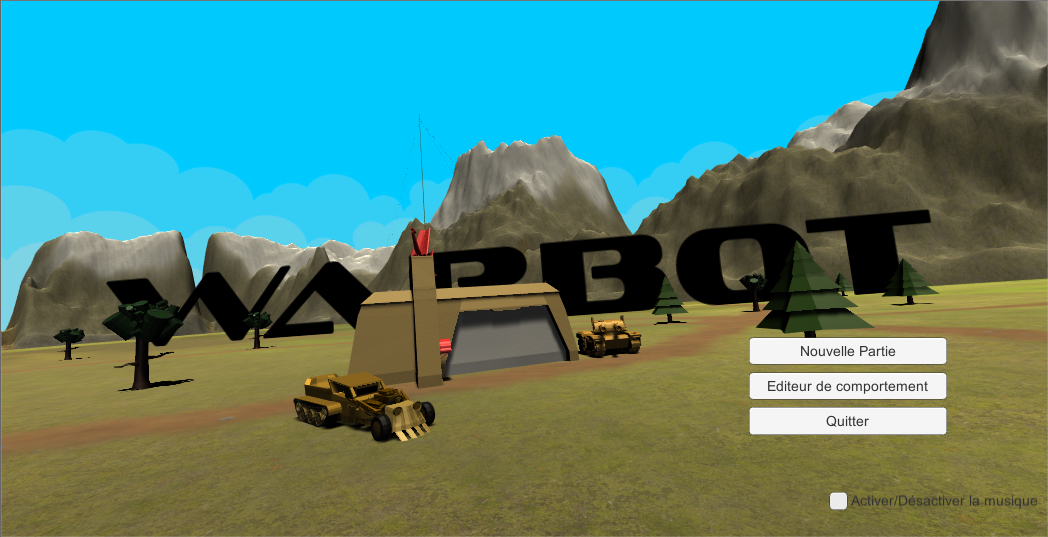
\includegraphics[scale=0.50]{MainScreenOld}
	\caption{Menu Principal, Ancienne Interface}
\end{figure}

\subsection{Editeur de comportement}
L'éditeur de comportement se décompose en deux écrans distincts  : 
\begin{enumerate}
\item\textbf{Le menu Pause}
\paragraph{}
Ce menu apparaît par défaut lors d'une tentative d'accès à l'éditeur de comportement si aucune équipe n'existe. Il permet donc de créer une nouvelle équipe, en entrant son nom.\newline
De plus, il permet de revenir au menu principal, de lancer une nouvelle partie, de quitter le jeu, ou bien tout simplement de fermer ce menu pour accéder à l'éditeur de comportement.\newline
Ce menu est toutefois "caché". Pour y accéder, il faut appuyer sur la touche "ECHAP" du clavier pour le voir s'afficher.
\clearpage
\begin{figure}[h]
	\centering
		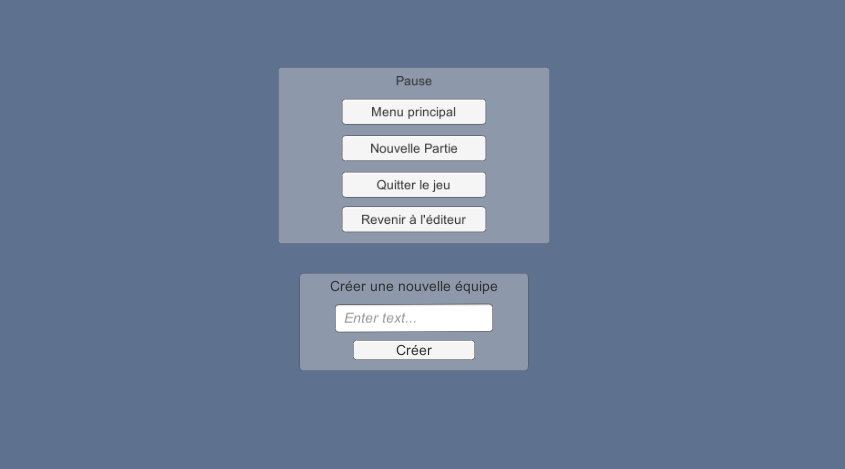
\includegraphics[scale=0.50]{PauseMenuOld}
	\caption{Menu Pause, Ancienne Interface}
\end{figure}


\item\textbf{L'éditeur en lui même}\newline
Nous avons maintenant devant nous un éditeur sobre. En haut à gauche se trouve le nom de l'équipe courante, ainsi que l’unité sur laquelle on va travailler.\newline
Juste en dessous, une liste de primitives, utiles à la création de comportement.\newline
Et enfin, à droite, la zone d'édition.

\begin{figure}[h]
	\centering
		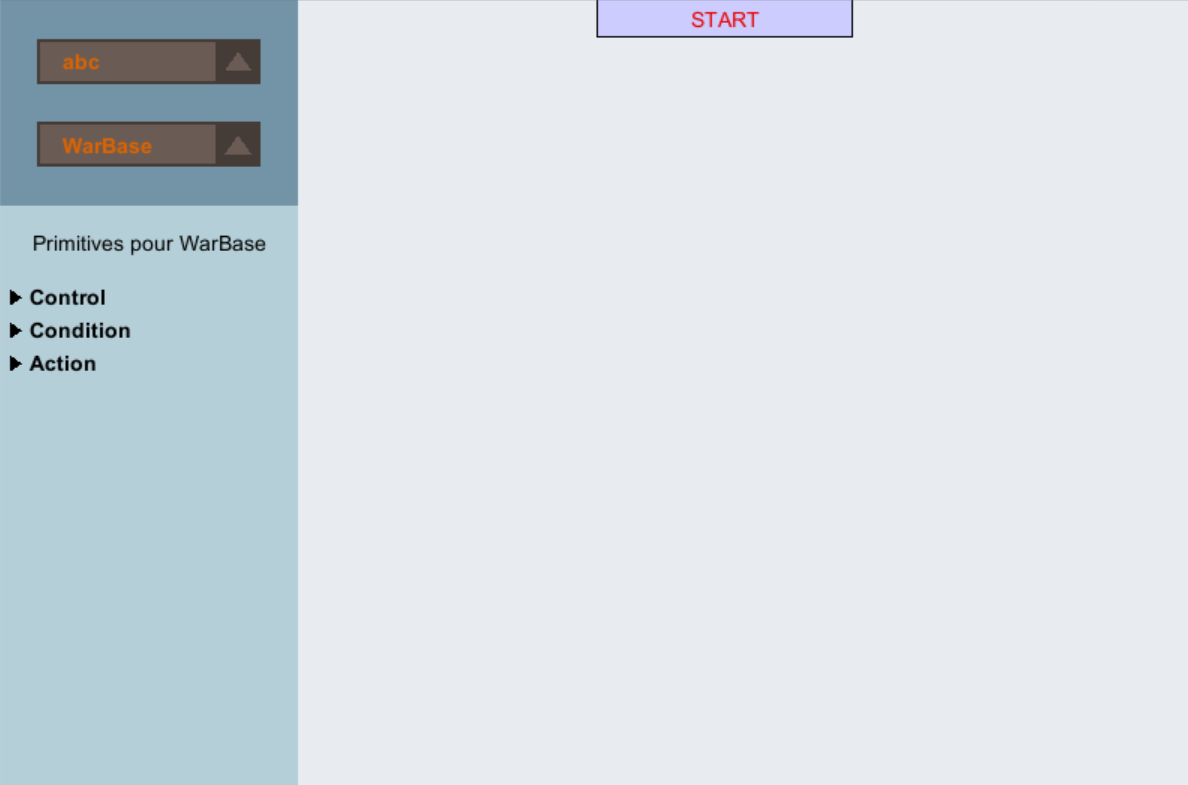
\includegraphics[scale=0.50]{BehaviorScreenOld}
	\caption{Editeur de Comportement, Ancienne Interface}
\end{figure}

\end{enumerate}


\subsection{La séléction des équipes}
Une fois le bouton "Nouvelle partie" cliqué, nous arrivons sur un nouvel écran, permettant de choisir les équipes qui vont participer, ainsi que le nombre de chacune de leurs unités qui commenceront directement en jeu.\newline
Cet écran permet également de revenir au menu principal, ou bien tout simplement de lancer la partie. Cette étape supplémentaire demandé à l'utilisateur ne nous paraissait pas spécialement utile. L'écran ne propose rien d'autre que la gestion des paramètres de partie. L'espace utilisé est moindre pour justifier l'affichage d'un nouvel écran.

\begin{figure}[!h]
	\centering
		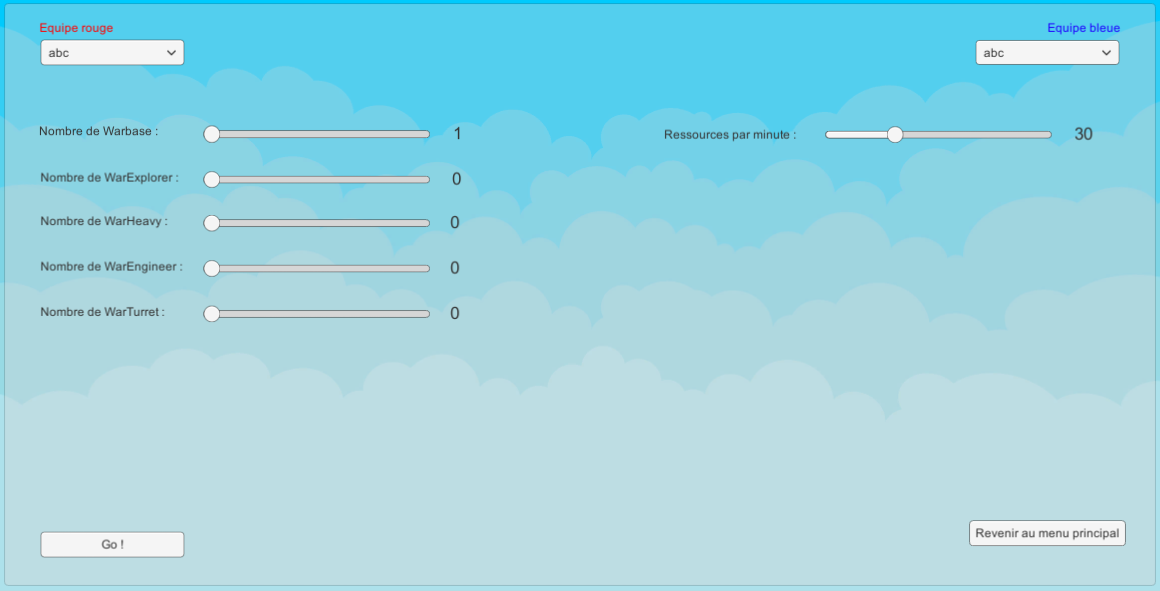
\includegraphics[scale=0.50]{SettingsOld}
	\caption{Sélection des équipes, Ancienne Interface}
\end{figure}

\subsection{Améliorations envisagées}
\paragraph{}
Les fonctionnalités primordiales au bon fonctionnement du jeu sont disponibles :
\begin{itemize}
\item La sélection de l’équipe et de toutes les unités 
\item La liste des primitives concernant l’unité sélectionnée 
\item La description et le placement des primitives 
\item La création et l’édition de l’architecture de subsomption via l’aire de jeu
\end{itemize}

Ceci dit, nous souhaitions revoir quelques points. \newline
Premièrement, nous voulions que tout soit le plus intuitif possible pour l'utilisateur. Il fallait que toutes les fonctionnalités proposées soient accessibles facilement. Par exemple, la création d'équipe n'est pas évidente à trouver. Il faut passer par un menu "caché" (appuyer sur la touche "ESC" depuis l'éditeur de comportement) pour pouvoir y accéder. Nous voulions éviter ce genre de problèmes. Des petits soucis d'optimisations étaient également présents, tel que la difficulté d'aimanter deux blocs. Si on ne posait pas le bloc à un endroit précis, il disparaissait. Il fallait alors le sélectionner à nouveau dans la liste de primitives, et retenter l'opération. A force, cela peut vite devenir redondant.
\newline
\smallbreak
Bien que l'éditeur soit fonctionnel, il nous paraissait assez austère, pas suffisamment "User Friendly". L'utilisateur passe la majeur partie de son temps sur cet écran. Il fallait donc qu'il soit le plus agréable  possible à l’œil, pour ne pas lasser l'utilisateur, et lui donner envie de passer du temps dessus.\newline \smallbreak
Enfin, l'absence totale de paramètres nous a semblé dommage. On ne peut qu'activer ou désactiver le son, mais pas régler le volume. L'utilisateur ne sait pas comment gérer les équipes qui vont participer, ainsi que leur nombre d'unités, avant d'avoir cliqué sur Nouvelle Partie. Ce comportement ne parait pas intuitif. L'ajout d'une gestion des paramètres nous semblait donc indispensable.

Nous avons donc décidés de revoir l'organisation de l'interface depuis le début. Adapter cette interface n'aurait pas été justifié, car trop de changements étaient à prévoir, tant sur le point technique que graphique.\newline
Nous souhaitions également proposer une cohésion graphique entre chaque écran, et le jeu lui-même.


\section{Nouvelle Interface}
Nous devions repartir d'une toute nouvelle interface, tout en s'inspirant de l'ancienne. Comme dit précédemment, nous voulions éviter au maximum les écrans intermédiaires qui n'étaient pas indispensables.
Nous avons donc décidé de mettre en place deux écrans : le menu principal,  et l'éditeur de comportement. Dans le menu principal se trouve une fenêtre "pop-up" dédiée à la configuration des paramètres. D'autres fenêtres "pop-up" peuvent apparaître, mais elles n'ont que pour but d'effectuer une vérification de l'action émise par l'utilisateur. Par exemple, confirmer la suppression d'une équipe, confirmer la fermeture du jeu, etc...

\subsection{Menu Principal}
Le menu principal donne accès aux options majeures du jeu. Ce menu doit contenir toutes les fonctionnalités dont l'utilisateur peut avoir besoin pour gérer le lancement d'une partie, sans avoir à accéder à l'éditeur de comportement.
Cela comporte donc les paramètres de la partie, le choix des équipes, du nombre d'unités, de la carte, etc... \newline
\begin{figure}[!h]
	\centering
		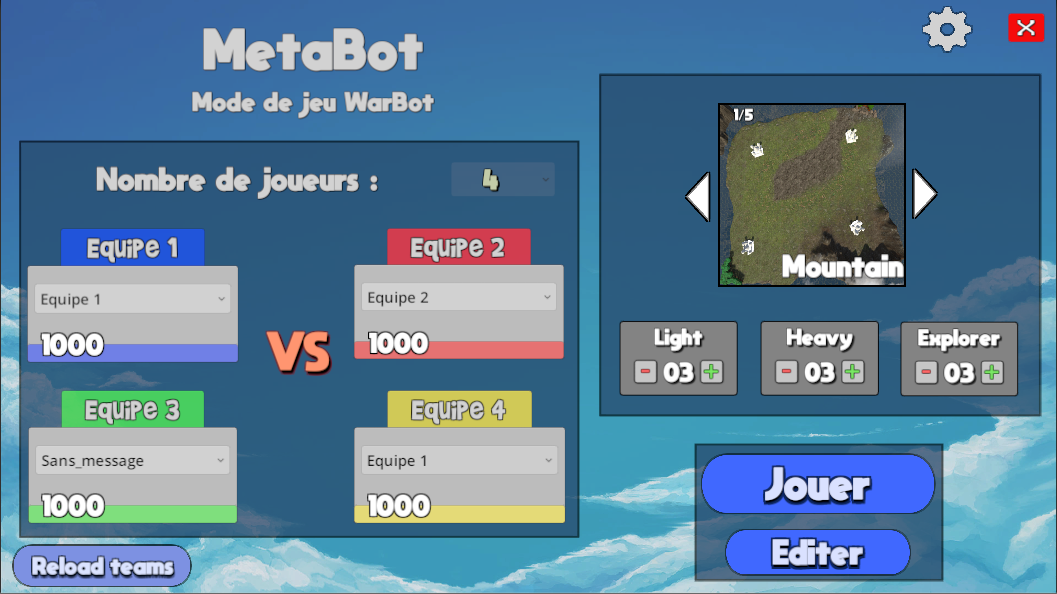
\includegraphics[scale=0.50]{MenuPrincipal}
	\caption{Menu Principal, Nouvelle Interface}
\end{figure}
Passons en revue tous les éléments présents sur cet écran.
\subsubsection{Lancer une Partie}
Le bouton "Jouer" permet de lancer une partie du jeu MetaBot. Le lancement de la partie prend en compte le mode de jeu sélectionné, les équipes choisies, le nombre de chaque unités en début de partie, le nombre de ressources maximum (nombre de ressource présentes en jeu au même moment), et la carte de jeu. Un script rattaché à ce bouton va donc se charger d'aller récupérer toutes ces informations stockées dans les différents "GameObject" de notre scène.

\begin{lstlisting}[language={[Sharp]C},label={lst:StartGame()}, caption= Extrait du code de PlayButton.cs]

public void StartGame()
    {
        
        nbPlayers = int.Parse(_numberplayerDropDown.GetComponent<Dropdown>().captionText.text);
        XMLWarbotInterpreter interpreter = new XMLWarbotInterpreter();

        GameObject gameManager = GameObject.Find("GameManager");
        string gamePath = Application.streamingAssetsPath + "/teams/" + gameManager.GetComponent<GameManager>()._gameName + "/";
        
        gameManager.GetComponent<TeamManager>()._teams = new List<Team>();

        for (int i = 0; i < nbPlayers; i++)
        {
            Team team = new Team();
            team._color = _DropDownList[i]._teamColor;
            team._name = _DropDownList[i]._teamName;//.Replace("_", " ");
            team._unitsBehaviour = interpreter.xmlToBehavior(gamePath + team._name, gamePath);
            gameManager.GetComponent<TeamManager>()._teams.Add(team);
        }

        GameManager setting = gameManager.GetComponent<GameManager>();
        setting.SetSetting();

        //
        StartCoroutine(AsynchronousLoad(setting._gameSettings._indexSceneMap));
    }
}
\end{lstlisting}


\subsubsection{Bouton Éditeur de Comportement}
Le bouton "Editer" permet d'accéder à l'éditeur de comportement, qui permettra à l'utilisateur, entre autres, de créer et/ou modifier le comportement de ses équipes.
\subsubsection{Bouton Paramètres}
L'icône en forme d'engrenage représente le bouton paramètres. Il va permettre d'afficher la fenêtre "pop-up" qui contient tous les paramètres du jeu.
\subsubsection{Choisir le nombre d'équipe}
Nous avons la possibilité de choisir le nombre d'équipes participant à la partie. Les valeurs sont dans un menu déroulant et vont de 2 à 4. Sa valeur courante sera récupérée par le script StartGame() (cf Listing 4.1).\newline
En fonction du nombre d'équipes choisies, le nombre de cadres d'équipe changera.
\subsubsection{Choisir les équipes}
Dans le cadre de chaque équipe se trouve un menu déroulant avec les noms de toutes les équipes présentes dans les fichiers du jeu. On peut donc en sélectionner une pour qu'elle participe à la prochaine bataille.
Pour récupérer toutes les équipes existantes, nous allons chercher la liste comprenant le nom de toutes les équipes.

\begin{lstlisting}[language={[Sharp]C},label={lst:Start()}, caption= Extrait du code de TeamMenuHUD.cs]
[...]
string team = GameObject.Find("GameManager").GetComponent<TeamManager>()._teams[_idPlayer]._name;
            for (int i = 0; i < _teamDropDown.options.Count; i ++)
            {
                if (_teamDropDown.options[i].text.Equals(team))
                {
                    _teamDropDown.value = i;
                }
            }
[...]
\end{lstlisting}
\smallbreak
De plus, à coté du nom de l'équipe, on retrouve aussi son score (ELO). Pour son affichage, nous récupérons le score associé à l'équipe courante. La couleur du score dépendra de sa valeur. (rouge = score faible, bleu = score élevé)

\begin{lstlisting}[language={[Sharp]C},label={lst:Change()}, caption= Extrait du code de TeamMenuHUD.cs]
public void Change()
    {
        _teamName = _teamDropDown.captionText.text;
        _powerScoreText.text = TeamsPerformance.GetTeamElo(_teamName).ToString();
        _powerScoreText.color = ColorElo(TeamsPerformance.GetTeamElo(_teamName));
    }
\end{lstlisting}
\subsubsection{Bouton "Reload Team"}
Ce bouton permet de recharger les équipes. L'intérêt est de permettre à l'utilisateur d'ajouter manuellement au dossier des équipes des nouveaux fichiers d'équipes, et de les voir apparaître en cliquant simplement sur ce bouton, sans avoir à relancer le jeu.
Pour permettre cela, nous devons aller chercher le dossier contenant les fichiers des équipes, le parcourir, et mettre à jour notre liste d'équipes.

\begin{lstlisting}[language={[Sharp]C},label={lst:Updating()}, caption= Extrait du code de GameSettingsScript.cs]
teams = new List<string>();
        string[] fileEntries = Directory.GetFiles(gamePath);
        foreach (string s in fileEntries)
        {
            string team = stringDifference(s, gamePath);
            if (team.Contains(".wbt") && !team.Contains(".meta"))
            {
                teams.Add(team);
            }
        }
\end{lstlisting}

\subsubsection{Choisir carte de jeu}
On peut directement choisir le lieu de la partie en cliquant sur les flèches de part et d'autre de l’aperçu de la carte. Il existe pour le moment cinq cartes: Moutain, Plain, Simple, Desolate et Garden. Chaque changement de carte mettra à jour le nom affiché, ainsi que le visuel de l'aperçu de la carte. Pour cela, il suffit de récupérer le nom de la carte sélectionnée, ainsi que son visuel associé, puis de les afficher.

\begin{figure}[!h]
	\centering
		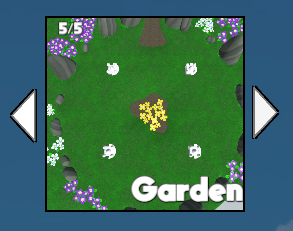
\includegraphics[scale=0.80]{ChoiceMap}
	\caption{Aperçu de la sélection de carte}
\end{figure}
\subsubsection{Choisir nombre de départ de chaque unité}
En dessous de l’aperçu de la carte, il y a les noms des unités existantes. Sous ces noms, le chiffre indique le nombre de ce type d'unité présent au lancement de la partie. On peut incrémenter ou décrémenter ce chiffre à l'aide des boutons "+" et "-" à coté de celui-ci. A chaque clic sur le bouton "+", on incrémente la variable "number" associée à l'unité, et inversement avec "-", dans la limite du possible ( c'est-à-dire tout en vérifiant que la valeur maximale du nombre d'unités possible ne soit pas dépassé).

\begin{lstlisting}[language={[Sharp]C},label={lst:Add()}, caption= Extrait du code de UnitSettingMenu.cs]
_number = Mathf.Min(_maxNumber, _number + 1);
_unitCounter.text = _number.ToString("00");
\end{lstlisting}

\begin{figure}[!h]
	\centering
		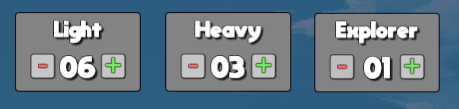
\includegraphics[scale=0.80]{NumberUnits}
	\caption{Choix du nombre d'unités}
\end{figure}

\subsubsection{Barre de Chargement}
Quand on lance une partie, une barre de chargement apparaît et indique l'avancement du chargement de la partie.
Ceci est une fonction qui utilise "AsyncOperation". La variable ao va contrôler l'avancée du chargement de la scène jeu.
Nous allons récupérer cette valeur, et la passer à notre slider.
La scène se chargera qu'une fois la progression de l'AsyncOperation terminée.
De cette manière, l'utilisateur peut voir où en est le chargement de sa partie.

\begin{lstlisting}[language={[Sharp]C},label={lst:Add()}, caption= Extrait du code de UnitSettingMenu.cs]
IEnumerator AsynchronousLoad(int scene)
    {
        loadingScreenBar.SetActive(true);
        yield return null;
        AsyncOperation ao = SceneManager.LoadSceneAsync(scene);
        ao.allowSceneActivation = false;
        while (!ao.isDone)
        {
            sliderLoad.value = ao.progress;
            if (ao.progress == 0.9f)
            { 
               sliderLoad.value = 1f;
               ao.allowSceneActivation = true;
            }
            yield return null;
        }
    }
\end{lstlisting}



\subsection{Menu des Paramètres}
Ce menu regroupe les paramètres de jeu. 

\subsubsection{Changer le Volume de la musique}
Ce slider indique le niveau sonore de la musique. On peut le modifier en cliquant dessus et en déplaçant la valeur de 0 jusqu’à 100. 0 correspond à un arrêt de la musique et 100 au volume maximal. De plus, le volume sonore dans le menu est le même dans l'éditeur de comportement et dans le jeu lui même.
La valeur de notre slider affectera directement la valeur de notre AudioSource.
\smallbreak
\begin{figure}[!h]
	\centering
		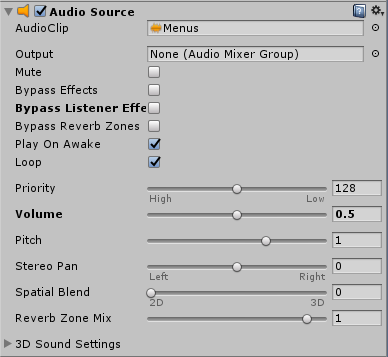
\includegraphics[scale=0.60]{AudioSource}
	\caption{Aperçu de l'AudioSource, dans l'Inspector}
\end{figure}

\subsubsection{Choisir le nombre de ressource maximales dans le jeu}
Dans cette case, on peut entrer un chiffre entier qui indiquera le nombre maximum de ressources présentes simultanément en jeu.
\smallbreak
\begin{figure}[!h]
	\centering
		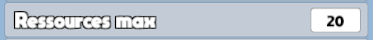
\includegraphics[scale=0.80]{RessourcesMax}
	\caption{Choix du nombre maximal de ressources}
\end{figure}
\subsubsection{Choisir le mode de jeu}
Ce menu déroulant permet de choisir le mode de jeu de la prochaine partie. Il y a actuellement deux modes, le mode MetaBot et le mode RessourceRace. Le mode MetaBot est le mode classique. Le mode RessourceRace est une course aux ressources. La première équipe à atteindre le nombre de ressources fixé par le joueur gagne.

Si le mode choisi est RessourceRace alors deux autres paramètres apparaissent:
\begin{itemize}
\item le temps imparti
\item le nombre de ressources à atteindre pour gagner.
\end{itemize}

\begin{figure}[!h]
	\centering
		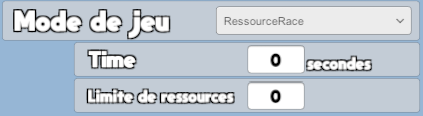
\includegraphics[scale=0.80]{ManuelJeu/ModeJeuRessourceRace}
	\caption{Paramètres RessourceRace}
\end{figure}

\subsubsection{Choisir la langue}
Les boutons en forme de drapeau indiquent les langues disponibles pour le jeu. Pour changer de langue, il suffit d'appuyer sur le drapeau voulu et de cliquer sur "Valider".
La traduction de chaque texte présent dans l'interface se fait grâce à des fichiers .yml, et .txt.
L'appel au traducteur permet ce changement. 
Nous ne traiterons pas en détail son fonctionnement, car il concèrne la partie Interpréteur.
\begin{lstlisting}[language={[Sharp]C},label={lst:ChangementLangue(string newLangage)}, caption= Extrait du code de ChangeLanguage.cs]
public void ChangementLangue(string newLangage)
    {
        GameObject.Find("GameManager").GetComponent<LangageLoader>().changeLanguage(newLangage);
        GameObject.Find("GameManager").GetComponent<Traducteur>().langue = newLangage;
        

        string[] lines = System.IO.File.ReadAllLines(Application.streamingAssetsPath+"/properties.yml");
        int cpt = 0;
        foreach (string line in lines)
        {
            if (line.Contains("Language"))
            {
                string[] tmp = line.Split('=');
                tmp[1] = newLangage;
                lines[cpt] = tmp[0] + "=" + tmp[1];
                break;
            }
            cpt++;
        }
        System.IO.File.WriteAllLines(Application.streamingAssetsPath+"/properties.yml", lines);
    }
\end{lstlisting}

\subsubsection{Bouton Retour}
Ce bouton permet de retourner à l'écran du menu principal.
Contrairement au bouton "Appliquer", ce bouton n'applique aucun changement effectué par l'utilisateur.

\subsubsection{Bouton Valider}
Ce bouton valide les paramètres définis précédemment et revient au menu principal en ayant appliqué ces paramètres.

\begin{lstlisting}[language={[Sharp]C},label={lst:ApplySettings()}, caption= Extrait du code de SettingsButton.cs]
public void ApplySettings()
    {
        setButtonActive();
        manageVolume();
        changeLanguage.ChangementLangue(language);
        changeGameMode();
        if(numberResources() == 0)
        {
            numberResources();
        }
        else
        {
            return;
        }
        window.SetActive(false);
    }
\end{lstlisting}

On peut apercevoir dans cette méthode, qu'elle appelle une méthode spécifique pour chaque paramètre modifiable.
Elle s'occupe donc d'appliquer chacune des modifications effectuées, via l'appel de la fonction adéquate.

\subsubsection{Bouton Quitter}
Ce bouton ouvre une boite de dialogue demandant à l'utilisateur s'il veut vraiment quitter le jeu. Il peut ainsi choisir de revenir sur le menu principal ou fermer le jeu.


\subsection{Editeur de Comportement}
\paragraph{}
Pour la refonte de l'éditeur de comportement, ce qui nous a paru le plus optimal fut de repartir d'une interface vierge. Nous avions identifié un nombre trop important de changements à effectuer pour justifier des modifications de l'ancienne interface.
Nous avons commencé par faire un croquis de deux interfaces potentielles.
\begin{figure}[!h]
	\centering
		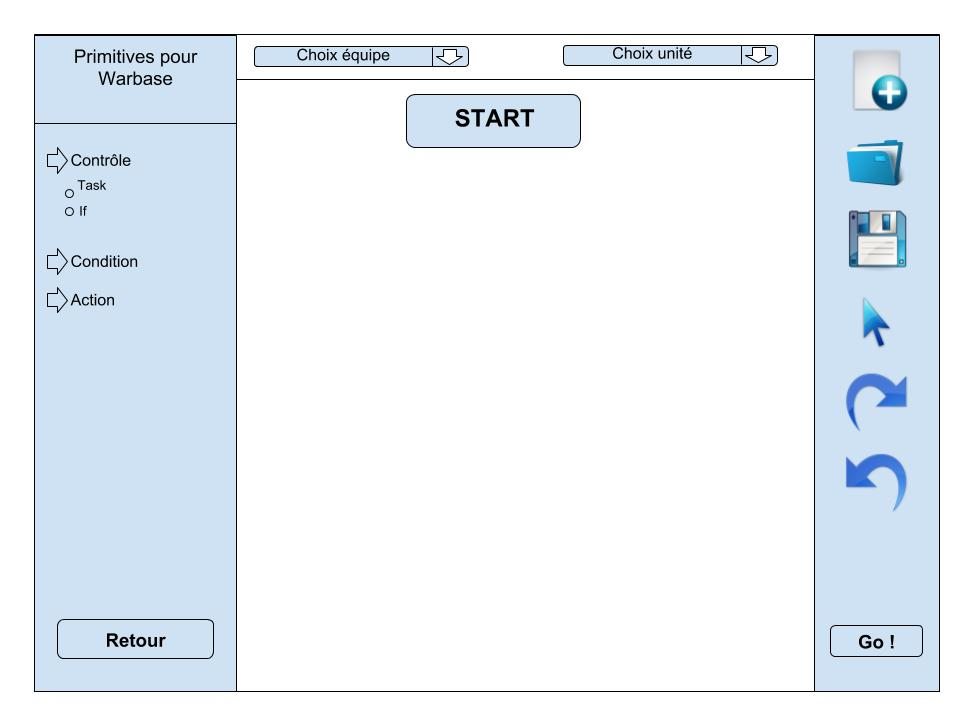
\includegraphics[scale=0.35]{ConceptionGraphique1}
	\caption{Première ébauche}
\end{figure}


\paragraph{}
Le premier modèle s'appuie sur l'esprit de l'ancienne interface, avec le panneau de contrôles fortement similaire. Cependant, après concertation lors d'une réunion, nous avons écarté ce modèle, car il ne semblait pas optimisé. La barre d'outils paraissait bien trop importante, et la zone d'édition de comportement s'en voyait restreinte.\newline
Quant au second modèle, il nous semblait organisé de manière plus logique, et intuitive. Toutes les options et choix se trouvent à gauche de la fenêtre, alors que la partie droite se consacre à l'édition du comportement.\newline
Nous avons donc décidé de partir sur ce modèle.

\begin{figure}[!h]
	\centering
		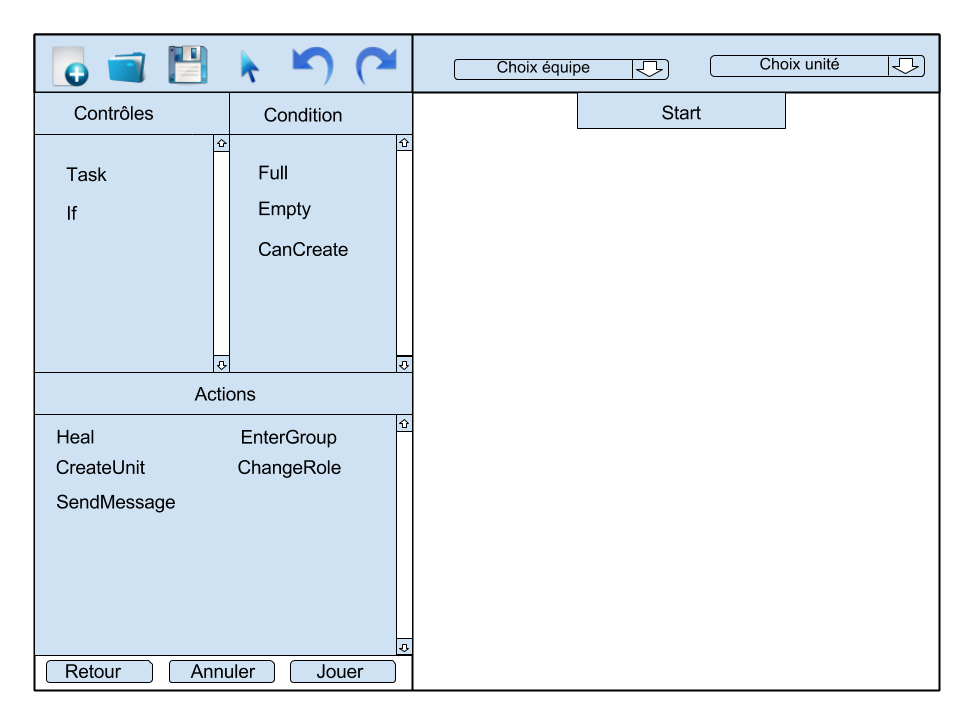
\includegraphics[scale=0.35]{ConceptionGraphique2}
	\caption{Seconde ébauche}
\end{figure}


\paragraph{}
Au fur et à mesure de nos avancées, de nouveaux éléments ont pris place dans l'interface. A force d'ajouter des informations et fonctionnalités, nous avons dû légèrement retravailler l'aspect global de l'écran, pour gagner en cohésion, et en ergonomie.
En voici un aperçu :
\clearpage
\begin{figure}[!h]
	\centering
		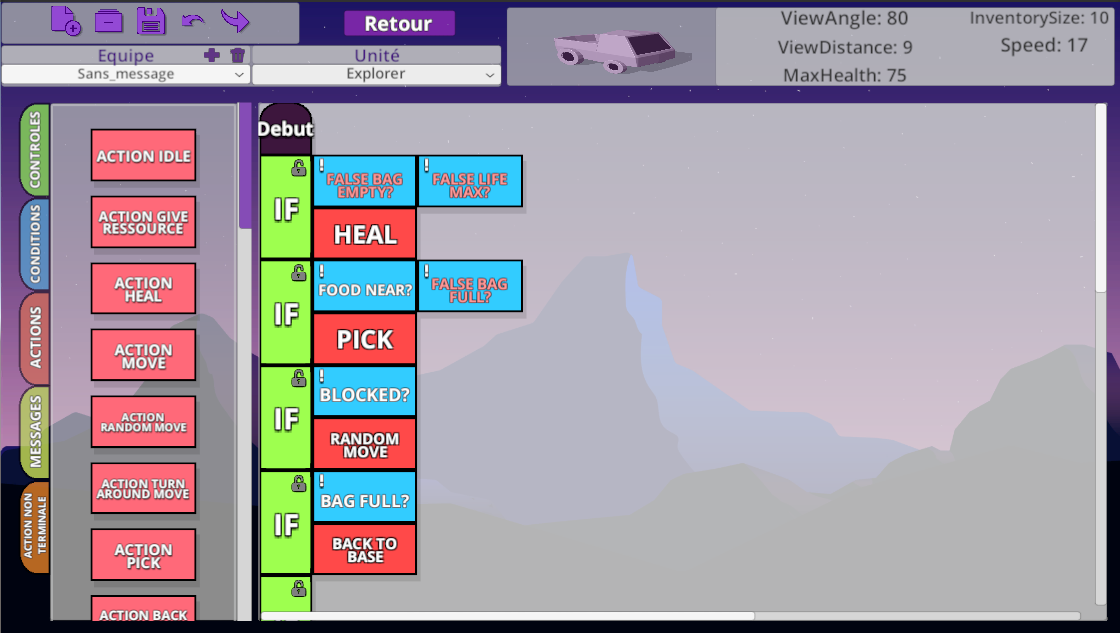
\includegraphics[scale=0.50]{InterfaceFinale}
	\caption{Interface Finale}
\end{figure}
% ToolBox %
\subsubsection{ToolBox}
La ToolBox est le panneau en haut à gauche de l'interface, regroupant des actions classiques, telles que la sauvegarde de fichier, la création d'un nouveau comportement, etc...

\begin{figure}[!h]
	\centering
		
\includegraphics[scale=0.50]{ToolBox}
	\caption{ToolBox, Editeur de comportement}
\end{figure}

\begin{enumerate}[label=\Alph*)]
\item\textbf{Bouton Nouveau Comportement} \newline
Ce bouton permet de commencer la création d'un nouveau comportement pour l'unité de l'équipe courante. Cela permet de repartir à zéro, lorsque notre comportement courant ne nous satisfait pas, et nous évite de devoir retirer chaque pièce manuellement.
\item\textbf{Bouton Chargement Comportement} \newline
Ce bouton permet de charger le comportement de l'unité actuellement sélectionnée dans le DropDown prévu à cet effet.
La première chose à faire est d'effacer le comportement actuellement chargé, s'il existe.
A l'aide du path, et du nom de l'équipe, nous allons pouvoir appeler une méthode présente dans l’interpréteur, pour transformer le fichier .xml correspondant à l'équipe courante, en un comportement, qui sera stocké dans un dictionnaire.\newline
Nous allons ensuite récupérer la position de la pièce "StartPuzzle", pour pouvoir placer les pièces correctement dans l'éditeur. Nous avons donc notre point de départ.\newline 
Il ne reste plus qu'à placer les pièces. Nous allons donc récupérer la liste d'instructions associée à chaque unité, et placer chaque instruction dans leur ordre d'apparition. (Un "if" pour commencer, suivi de sa ou ses conditions, suivies d'une ou plusieurs actions)\newline
Pour finir, on réinitialisera la scrollbar de l'éditeur, pour permettre à l'utilisateur de voir directement le début du comportement.\newline
\textit{Voir Annexes pour le script}
\item\textbf{Bouton Sauvegarde du Comportement} \newline
Ce bouton sauvegarde le comportement de l'unité de l'équipe courante. Si l'on change d'unité dans la même équipe sans sauvegarder, alors le comportement de l'unité précédente sera perdu.\newline
Voyons de plus près deux de ses fonctions primordiales au bon fonctionnement du script :

Nous allons créer un comportement, copiant le comportement présent dans l'éditeur. Pour commencer, nous allons répertorier toutes les pièces "If" présentes. Ensuite, pour chaque pièce If de la liste, nous allons créer l'instruction comprenant les conditions et actions, grâce à l'interpréteur.\newline
\begin{lstlisting}[language={[Sharp]C},label={lst:createBehavior()}, caption= Extrait du code de SaveFile.cs]
public void createBehavior()
    {
        GameObject startPuzzle = GameObject.FindGameObjectWithTag("StartPuzzle");
        GameObject ifpuzzle = startPuzzle.GetComponent<StartPuzzleScript>().ifPuzzle;
        while (ifpuzzle != null && ifpuzzle.activeSelf == true)
        {
            // Crée l'instruction (conditions + une/des actions) correspondate au If courant
            listBehavior.Add(ifpuzzle.GetComponent<IfPuzzleScript>().createInstruction());
            ifpuzzle = ifpuzzle.GetComponent<IfPuzzleScript>().puzzleIfObject;
        }
        createXML();
        Debug.Log("Saving file done !");
        listBehavior.RemoveRange(0, listBehavior.Count);
    }
\end{lstlisting}
Une fois chaque instruction créée pour chaque "If", nous pouvons appeler la fonction createXML().\newline
\item\textbf{createXML()} :  \newline
Appelle la fonction behaviorToXml(), présente dans l'interpréteur, qui prend en paramètres le nom de l'équipe courante, le chemin où écrire le fichier .xml, le nom de l'unité, et la liste d'instructions correspondante.
\begin{lstlisting}[language={[Sharp]C},label={lst:createXML()}, caption= Extrait du code de SaveFile.cs]
public void createXML()
{
    //récupération de l'unité actuellement traitée et de l'équipe
    string teamName = team.captionText.text;
    string unitName = unit.captionText.text;
    string path = Application.dataPath + "/StreamingAssets/" + Constants.teamsDirectory + Constants.gameModeWarBot;
    if(teamName != "")
    {
        XMLWarbotInterpreter interpreter = new XMLWarbotInterpreter();
        interpreter.behaviorToXml(teamName, path, unitName, listBehavior);
    }        
}
\end{lstlisting}

\item\textbf{Bouton "Undo"} \newline
Ce bouton va permettre d'annuler la création ou la suppression d'une pièce. Lors de la création d'une pièce, cette pièce sera ajoutée dans une liste "listPieces", qui nous permettra de garder une trace de l'ordre dans lequel les pièces ont été créées.
\smallbreak
Cette fonction requiert une liste de pièces non vide pour fonctionner, c'est donc ce que l'on va vérifier en premier. Si la liste "listPieces" n'est pas vide, alors on stocke la dernière pièce de cette liste dans une variable "pieceToUndo".\newline
Maintenant, il faut déterminer quelle action utilisateur nous devons annuler (création ou suppression).\newline
Si "pieceToUndo" est active, alors nous devons simuler sa suppression, en la passant inactive. Il faudra également l'ajouter dans la liste "recoverList", qui a un comportement similaire à "listPieces", pour reconstituer une annulation.\newline
Si, en revanche, la pièce est inactive, il faut alors la faire réapparaitre à l'écran, en la passant en active.

\begin{lstlisting}[language={[Sharp]C},label={lst:Undo()()}, caption= Extrait du code de createPuzzle.cs]
public void Undo()
{

    if( cptObjects > 0 ) {
		
        pieceToUndo = (GameObject)listPieces[cptObjects - 1];
        // Si la pièce à "undo" est une pièce IF, on oublie pas de mettre à jour le compteur de pièces IF
        if (pieceToUndo.tag == "IfPuzzle") {
            cptIfPuzzle = numberIfPuzzle() - 1;
        }
            // Si la pièce à "undo" est active, alors on la masque, on l'ajoute à la liste redo et on met a jour le compteur d'objet
            if(pieceToUndo.activeSelf == true) {
            recoverList.Add(pieceToUndo);
            pieceToUndo.SetActive(false);
            cptObjects--;
        }
        // Si la pièce à "undo" est inactive, alors on l'active et on change son ordre dans la liste des pièces
        else if(pieceToUndo.activeSelf == false) {
            pieceToUndo.SetActive(true);
            listPieces.Remove(pieceToUndo);
            listPieces.Insert(0,pieceToUndo);
        }

        cptUndo = recoverList.Count;
    }
}
\end{lstlisting}	
\item\textbf{Bouton "Redo"} \newline
Ce bouton permet de restituer une annulation préalablement faite. Lorsqu'on clique sur le bouton Annuler, on va conserver l'action annulée dans une liste, qui nous servira donc à la restituer lors d'un clic sur le bouton Redo.
\begin{lstlisting}[language={[Sharp]C},label={lst:Redo()}, caption= Extrait du code de createPuzzle.cs]
// Restitue la dernière pièce de la liste recoverList
public void Redo()
{
    if( recoverList.Count > 0 ) {
        GameObject pieceToRedo = (GameObject)recoverList[cptUndo - 1];
        if (pieceToRedo.tag == "IfPuzzle") {
            cptIfPuzzle = numberIfPuzzle() + 1;
        }
        pieceToRedo.SetActive(true);
        recoverList.RemoveAt(cptUndo - 1);
        cptObjects++;
        cptUndo = recoverList.Count;        
    }
}
\end{lstlisting}	
\item\textbf{Bouton de retour au menu principal} \newline
Ce bouton ramène l'utilisateur au menu principal. Avant de cliquer dessus, il faut penser à bien sauvegarder le comportement en cours pour ne pas le perdre.
\end{enumerate}




% Equipe + Unité %
\subsubsection{Sélection des équipes / unités}
Ce cadre nous permet de sélectionner l'équipe et l'unité sur lesquels nous souhaitons travailler.
Chaque équipe est composée du même type d'unités. Deux boutons sont également disponibles, permettant de créer ou supprimer l'équipe couramment sélectionnée.
\begin{figure}[!h]
	\centering
		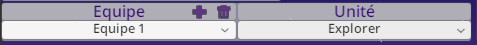
\includegraphics[scale=1]{SelectionTeamUnit}
	\caption{Sélection des équipes / unités}
\end{figure}

\begin{enumerate}[label=\Alph*)]
\item\textbf{Choix de l'équipe} \newline
Ce menu déroulant permet de choisir l'équipe sur laquelle on veut travailler. Un clic sur le menu déroule la liste, qui comprend le nom de toutes les équipes.
Cette liste est tenue à jour, dès que l'on ajoute une équipe, supprime une équipe, ou bien que l'on ajoute un fichier équipe à la main, et que l'on appuie sur le bouton "Reload team" du menu principal.
\item\textbf{Choix de l'unité} \newline
Ce menu déroulant permet de choisir l'unité de l'équipe sur laquelle on va opérer les changements de son comportement.
Lorsqu'une unité est sélectionnée, son comportement, s'il existe, sera dynamiquement chargé dans l'éditeur, grâce à la fonction createBehaviorFromXML() du script LoadFile (détaillé en annexe).\newline
Il faut aussi charger les statistiques et le modèle e l'unité sélectionnée, toujours dynamiquement. Pour ça, nous allons faire appel à la méthode ReadStats() du script StatsLoader.cs, qui nous permettra à la fois d'afficher les statistiques de l'unité sélectionnée, mais aussi son modèle 3D.
Voici un exemple qui concerne l'unité "Base" :

\begin{lstlisting}[language={[Sharp]C},label={lst:ReadStats()()}, caption= Extrait du code de StatsLoader.cs]
[...]
// Lecture des statistiques de la base
            else if (unitName == "Base" && line.Contains("Base"))
            {
                readStatsFile(unitName, reader, statBase);
                imageUnit.sprite = baseSprite.sprite;
                imageUnit.color = new Color(imageUnit.color.r, imageUnit.color.g, imageUnit.color.b, 255);
            }
[...]
\end{lstlisting}	
\item\textbf{Bouton Création d'équipe} \newline
Juste à droite des équipes se trouve un bouton en forme de "+", il permet de créer un nouvelle équipe. Si l'on clique dessus, une boite de dialogue s'ouvre et nous demande le nom de la nouvelle équipe. Pour qu'une équipe soit créée, il faut vérifier plusieurs choses. D'abord, il faut s'assurer que son nom ne contient que des caractères contenus dans a-zA-Z0-9. Nous empêchons également la création d'équipe dont le nom commence par le caractère "Espace". Ensuite, si le nom est valide, il faut que l'on vérifie si cette équipe n'existe pas déjà dans le dossier des équipes.\newline
Enfin, lorsque ces deux conditions sont respectées, alors il faut mettre à jour la liste des équipes, ainsi que le menu déroulant de sélection d'équipes.
\begin{lstlisting}[language={[Sharp]C},label={lst:validateName()}, caption= Extrait du code de CreateTeam.cs]
// Vérifie le nom d'équipe entré par l'utilisateur, pour empêcher l'utilisation de caractères spéciaux
    // Caractères acceptés : a-zA-Z0-9
    public void validateName()
    {
        string teamName = mainInputField.text;
        string path = Application.streamingAssetsPath + "/teams/TestBot/";

        List<int> listInt = new List<int>();
        for (int i = 0; i < teamName.Length; i++)
        {
            listInt.Add(Convert.ToInt32(teamName[i]));
        }

        for (int i = 0; i < listInt.Count; i++)
        {
            int result = listInt[i];
            if ((result > 90 && result < 97) || (result < 65 && result > 57) || (result < 48 && result > 32) || result > 122)
            {
                errorText.SetActive(true);
                Text error = errorText.GetComponentInChildren<Text>();
                error.text = "Nom invalide ! (a-zA-Z0-9)";
                return;
            }
            if (listInt[0] == 32) //&& result == 32)
            {
                errorText.SetActive(true);
                Text errorSpace = errorText.GetComponentInChildren<Text>();
                errorSpace.text = "Nom invalide ! (a-zA-Z0-9)";
                return;
            }
        }

        if(listInt.Count == 0)
        {
            errorText.SetActive(true);
            Text errorSpace = errorText.GetComponentInChildren<Text>();
            errorSpace.text = "Nom invalide ! (a-zA-Z0-9)";
            return;
        }

        foreach (string file in Directory.GetFiles(path))
        {
            string res = file.Replace(path, "");
            if (res == teamName + ".wbt")
            {
                errorText.SetActive(true);
                Text error = errorText.GetComponentInChildren<Text>();
                error.text = "L'équipe existe déjà !";
                return;
            }
        }

        if (!System.IO.File.Exists(Application.streamingAssetsPath + "/ELO/" + teamName + ".elo"))
        {
            File.Create(Application.streamingAssetsPath + "/ELO/" + teamName + ".elo").Dispose();
            File.WriteAllLines(Application.streamingAssetsPath + "/ELO/" + teamName + ".elo", new string[] { 1000 + "" });
        }

        dropOption.Add(teamName);
        teamDropDown.AddOptions(dropOption);
        XMLWarbotInterpreter interpreter = new XMLWarbotInterpreter();
        interpreter.generateEmptyFile(teamName, path);
        dropOption.Clear();
        errorText.SetActive(false);
        window.SetActive(false);
    }
\end{lstlisting}	

\item\textbf{Bouton Suppression d'équipe} \newline
Ce bouton permet de supprimer définitivement l'équipe courante. Une boite de dialogue demandera confirmation.
Pour supprimer une équipe, il nous suffit de supprimer les fichiers qui lui sont associés, dans le dossier contenant toutes les équipes. Il ne faut pas oublier de mettre à jour le menu déroulant de sélection des équipes, pour qu'elle cesse d'y apparaître.
\end{enumerate}


\subsubsection{Informations sur l'unité}
Ce cadre a un but purement informatif. Diverses informations concernant notre unité sont affichées. Ces informations sont chargées en temps réel.\newline
Si l'utilisateur sélectionne une nouvelle unité, sa représentation 3D ainsi que ses statistiques seront immédiatement affichées dans ce cadre.
\clearpage
\begin{figure}[h]
	\centering
		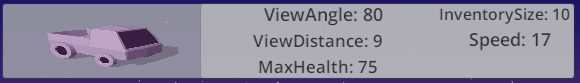
\includegraphics[scale=1]{StatsModel}
	\caption{Informations sur l'unité}
\end{figure}

\begin{enumerate}[label=\Alph*)]
\item\textbf{Affichage des statistiques de l'unité courante} \newline
Quand on choisit une unité, sur sa droite apparaît ses valeurs dans un cadre, cela correspond à ses statistiques. Cela va permettre à l'utilisateur d'adapter ses stratégies en fonction des statistiques de chaque unité.
Ces statistiques ne changent pas d'une équipe à l'autre, elles sont inhérentes à l'unité.
\item\textbf{Affichage du modèle 3D de l'unité courante} \newline
Dans le même cadre apparaît aussi le modèle 3D de l'unité courante. C'est l'apparence qu'aura l'unité en jeu.
\end{enumerate}


% Zone de création des comportements
\subsubsection{Liste des pièces}
\begin{enumerate}[label=\Alph*)]
\item\textbf{Boutons de choix de la catégorie de la pièce} \newline
Sur la gauche, de manière verticale, se trouve cinq noms de catégories qui sont les Contrôles, les Conditions, les Actions, les Messages et les Actions non terminales. En cliquant sur l'une de ces catégories, on affiche la liste des éléments de cette catégorie dans la zone directement à droite.
\item\textbf{Zone de sélection de la pièce suivant la catégorie} \newline
C'est dans cette zone qu’apparaît la liste des éléments des catégories de pièces de l'éditeur. La génération des modèles des pièces se fait de manière dynamique. Chaque type de pièce a un prefab associé. \newline
Un script contenant une méthode pour chaque type de pièces disponibles (Conditions, Actions, etc...), permet ce dynamisme. Voyons de plus près la gestion d'une des catégories de pièces (leur comportement est semblable).
\begin{itemize}
\item\textbf{UpdateCondition()} : Nous commençons par récupérer une structure UnitPerceptAction, contenant le nom d'une unité, ainsi que toutes les conditions, actions, et messages inhérents à l'unité.\newline
A partir de là, nous pouvons créer, à l'aide du prefab correspondant, une pièce, avec le label contenu dans notre structure.
Nous allons parcourir la structure pour créer toutes les pièces disponibles pour l'unité, et modifier leur placement, en leur ajoutant un vecteur, pour qu'elles ne se superposent pas.
\begin{lstlisting}[frame=single]
new Vector2(0, -button.GetComponent<RectTransform>().rect.height)+ deltaVect;
\end{lstlisting}
Dans cette fonction, nous nous occupons uniquement de la liste Conditions présente dans notre structure. Il y a une fonction pour chaque liste de la structure.
\end{itemize}
\item\textbf{createPuzzle.cs} : Lors de l'appel à ce script, nous récupérons le prefab et le label associé au type de pièce concernée. Par exemple, pour une pièce "Conditions", nous récupérerons le prefab des pièces "<Conditions">, ainsi qu'un label nommé "PERCEPT". Le traitement de ce label se fait dans le script ConditionEditorScript.cs.\newline
Nous plaçons ensuite la pièce créée 

\begin{itemize}
\item\textbf{create()} : Lors d'un clic sur le modèle de pièce que l'on veut ajouter au comportement courant, cette fonction est appelée. Une position par défaut est définie dans l'éditeur, qui déterminera où la pièce sera placée lors de sa création.\newline
A chaque pièce créée, nous l'ajoutons dans la liste listPieces, utilisée pour la fonction Annuler.
\end{itemize}
\begin{lstlisting}[frame=single]
GameObject puzzleClone = (GameObject)Instantiate(puzzle, GameObject.Find("MaskEditeur").transform);
if (puzzleClone.GetComponent<PuzzleScript>())
{
   puzzleClone.GetComponent<PuzzleScript>()._value = _label;
}
\end{lstlisting}

Les pièces sont présentes sous forme de cases avec leur nom à l'intérieur (certaines possèdent des menus déroulant pour choisir la valeur voulue une fois dans la zone d'édition). La couleur des pièces dépend de leur catégorie.
Les pièces peuvent être sélectionnées et déplacées dans la zone d'édition du comportement grâce au glissé/déposé (Drag \& Drop).
\end{enumerate}

\subsubsection{Editeur}
C'est dans cette zone de l'éditeur que l’utilisateur pourra créer et modifier les comportements des untiés de ses équipes.
Nous voulions cette zone la plus grande possible, et la plus épurée possible, pour rendre le processus de création vraiment optimal.
\clearpage
\begin{figure}[h]
	\centering
		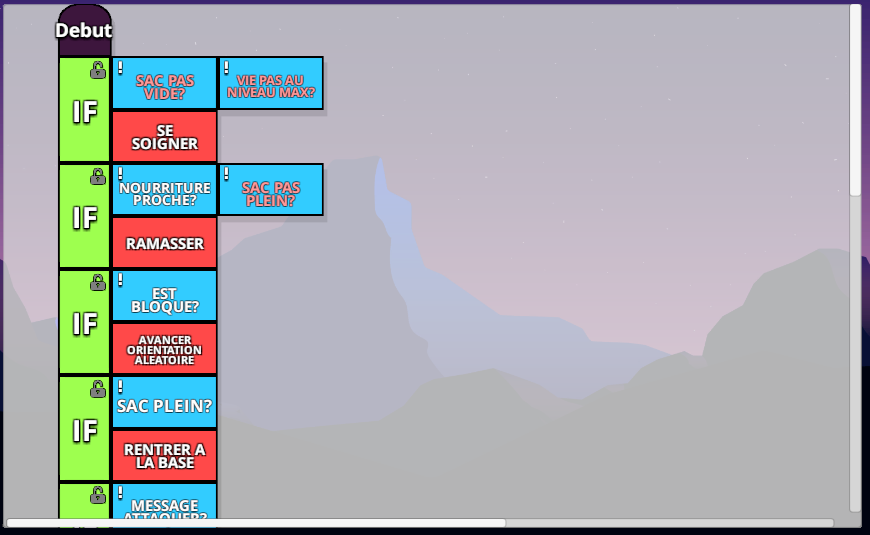
\includegraphics[scale=0.7]{ZoneEdition}
	\caption{Zone d'édition}
\end{figure}


\begin{enumerate}[label=\Alph*)]
\item\textbf{Zone éditeur de comportement de l'unité et de l'équipe courante} \newline
Dans cette zone arrivent les pièces venant de la zone de sélection. Elles se placent à l'aide du curseur de la souris sur une grille invisible. Si une pièce est valide, alors elle est colorée, sinon, elle est grise. Les pièces "IF" possèdent un cadenas dans le coin supérieur droit. Il permet de déplacer, en plus de la pièce IF, tout les éléments valides qui lui sont rattachés (hors IF). Les pièces de contrôles sont considérées comme valides si elles sont placées en dessous d'autres pièces du même type ou en dessous de la pièce "Start".\newline
Les autres pièces doivent se rattacher à des pièces de contrôle, en haut à droite pour les pièces Condition et en bas à droite pour les autres. Les pièces hors Contrôle sont ainsi valides lorsqu'elles sont au bon endroit, sur leur ligne, adjacentes au contrôle, ou adjacentes à une autre pièce du même type, valide. \newline \smallbreak

Voyons les scripts permettant cette gestion.

\begin{itemize}
\item\textbf{ManageDrapAndDrop.cs} : \newline 
Ce script s'occupe de la gestion du déplacement des pièces, ainsi que de leur placement, sur une grille aimantée.
\begin{itemize}
\item\textbf{OnMouseDrag()} : \newline
Une fois qu'un clic a été fait sur une pièce, cette fonction s'occupe de mettre à jour les coordonnées de la pièce, de telle sorte qu'elles soient égales à celles du pointeur de la souris. Pour valider les nouvelles coordonnées de la pièce, il faut appeler la fonction OnMouseUp().
\item\textbf{UpgradeGridPosition()} : \newline
Lorsque le clic de la souris est relâché (OnMouseUp), il faut mettre à jour la position de la pièce dans l'éditeur.
\begin{lstlisting}[frame=single]
posGridX = Mathf.Max((int)GameObject.Find("Editeur").GetComponent<RectTransform>().rect.x / 
  (int)widthPuzzle, (int)Mathf.Round(GetComponent<RectTransform>().localPosition.x / widthPuzzle));

posGridY = Mathf.Max((int)GameObject.Find("Editeur").GetComponent<RectTransform>().rect.y / 
  (int)heightPuzzle, (int)Mathf.Round(GetComponent<RectTransform>().localPosition.y / heightPuzzle));
\end{lstlisting}
\item\textbf{OnMouseUp()} : \newline
Cette fonction appelle la fonction UpdateGridPosition(), puis attribue à la pièce courante sa nouvelle position. Une fois cela fait, il faut vérifier que la nouvelle position de la pièce est toujours un emplacement valide, d'un point de vue comportement. La fonction appelle pour ça le script StartPuzzleScript.cs, que nous verrons plus bas.
\end{itemize}
\item\textbf{StartPuzzleScript.cs} : \newline
Ce script va nous permettre de vérifier si une pièce "If" est bien placée en dessous de la pièce Start.

\begin{itemize}
\item\textbf{UpdateAllValidPuzzles()} : \newline
Cette fonction, appelée dans ManageDragAndDrop.OnMouseUp(), va nous servir à vérifier si la position de la pièce "If" est correcte. Pour commencer, nous passons la variable booléenne "isValid" de toutes les pièces à false, puis nous allons vérifier leur placement.\newline
Pour se faire, nous allons appeler la fonction UpdatePuzzle() du script IfPuzzleScript.cs.\newline
Ensuite, si la pièce Start a bel et bien une pièce "If" juste en dessous d'elle, alors on passe la valeur isValid du "If" à true.
\end{itemize}

\item\textbf{IfPuzzleScript.cs} : \newline
Ce script s'occupe de vérifier le placement de toutes les pièces actuellement sur l'éditeur. Si leur positionnement n'est pas correct, leur couleur sera grise. Sinon, une pièce Contrôle sera verte, une pièce Condition sera bleue, une pièce Action Non Terminale sera orange, une pièce Action sera Rouge, et une pièce Message sera Jaune.
\begin{itemize}
\item\textbf{UpdateCondPuzzle()} : \newline
Cette fonction parcours toutes les pièces présentes sur l'éditeur. Si la pièce observée est une pièce de type Condition, et qu'elle est placée à droite d'une pièce "If", au niveau de sa première ligne, alors on l'attribue à une variable.

\begin{lstlisting}[frame=single]
if (currentGridPos + new Vector2(1,0) == puzzleGridPos && typePuzzle == PuzzleScript.Type.CONDITION)
\end{lstlisting}

\smallbreak
Cela nous permettra, dans UpdatePuzzle, de savoir que nous avons une pièce Condition placée à notre droite, sur la bonne ligne.
Le comportement des fonctions UpdateIfPuzzle() et UpdateActPuzzle est similaire. Le seul changement est la place dans l'éditeur. Une pièce "If" devra être située directement en dessous de notre "If" courant, et une pièce Action / Action non terminale / Message devra se trouver directement à droite de notre pièce "If", sur sa deuxième ligne.
\item\textbf{UpdatePuzzle()} : \newline
Cette fonction récupère les pièces adjacentes à notre pièce actuelle, à l'aide des scripts UpdateIfPuzzle(), UpdateCondPuzzle, UpdateActPuzzle(). Il met ensuite à jour les valeurs des pièces adjacentes, à savoir leur variable isValid, ainsi que leur variable NextPuzzle, qui leur permet de savoir quelle pièce leur est adjacente.

\end{itemize}
\end{itemize}
\end{enumerate}


\subsection{Élément dans le jeu}
\subsubsection{Réglage du volume du son}
En bas à droite de la fenêtre de jeu se trouve une icône de son et un slider. Le slider permet, comme dans le menu des paramètres, de modifier le volume du son. L’icône sert de bouton; si on le presse, le son passe à 0 et l’icône devient barrée. Si l'on appuie de nouveau, elle redevient classique, et le son est restitué à sa valeur précédente.
